\documentclass[unknownkeysallowed,usepdftitle=false]{beamer}
% unknownkeysallowed is needed for mac and the newer latex version -> is more picky than before...
\usetheme[headheight=1cm,footheight=2cm]{boxes}
%\usetheme{default}

\usepackage{inputenc}
\usepackage{default}
\usepackage{graphicx}
\usepackage{epsfig}
\usepackage{siunitx}
\usepackage{color}
\usepackage{ifthen}
\usepackage{ragged2e}

\setbeamertemplate{navigation symbols}{}%remove navigation symbols
\setbeamersize{text margin left=0pt,text margin right=0pt} % text and figures flush to edges

% some colors
\definecolor{grau}{gray}{.5}
\definecolor{slfcolor}{rgb}{0,0.5,0.8353}
\definecolor{wslcolor}{rgb}{0,0.4,0.4}

% setup links
\hypersetup{%
	%linkbordercolor=green,%
	colorlinks=false,%
	pdfborderstyle={/S/U/W 0},%
	%pdfpagemode=FullScreen,%
	pdfstartpage=4%
	}

% setup some fonts
\setbeamerfont{title}{series=\bfseries, size=\small}
\setbeamerfont{author}{size*={5pt}{0pt}}
\setbeamerfont{institute}{size*={3pt}{0pt}}
\setbeamerfont{bodytext}{size=\scriptsize}


% Title setup	
\title{Absolute Velocity Estimates from a Glider Mounted ADCP}
\author{Callum Rollo\inst{1} (\texttt{c.rollo@uea.ac.uk}) \and Karen J Heywood\inst{1} \and Rob Hall\inst{1} \and Alex Phillips\inst{2}}
\institute{\inst{1}University of East Anglia, Norwich, UK
\quad \inst{2}Marine Autonomous Robotics Systems group, Southampton UK}
% add title in headbox
\setbeamertemplate{headline}
{\leavevmode
\begin{beamercolorbox}[width=1\paperwidth]{head title}
  % LOGO
  \begin{columns}[t, totalwidth=\textwidth]
  \begin{column}[c]{1.05cm}
     
\includegraphics[height=1.05cm]{figure/graphic_egu_photo_yes.png}
  \end{column}
  % TITLE
   \begin{column}[c]{10.6cm}
   \centering \usebeamerfont{title} \textcolor{slfcolor}{\inserttitle} \\
   \centering \usebeamerfont{author} \color[rgb]{0,0,0} \insertauthor \\
   \vspace{-0.05cm}
   \centering \usebeamerfont{institute} \insertinstitute
  \end{column}
  % PICUTRE
  \begin{column}[c]{0.9cm}
    \hspace{0.005cm}
    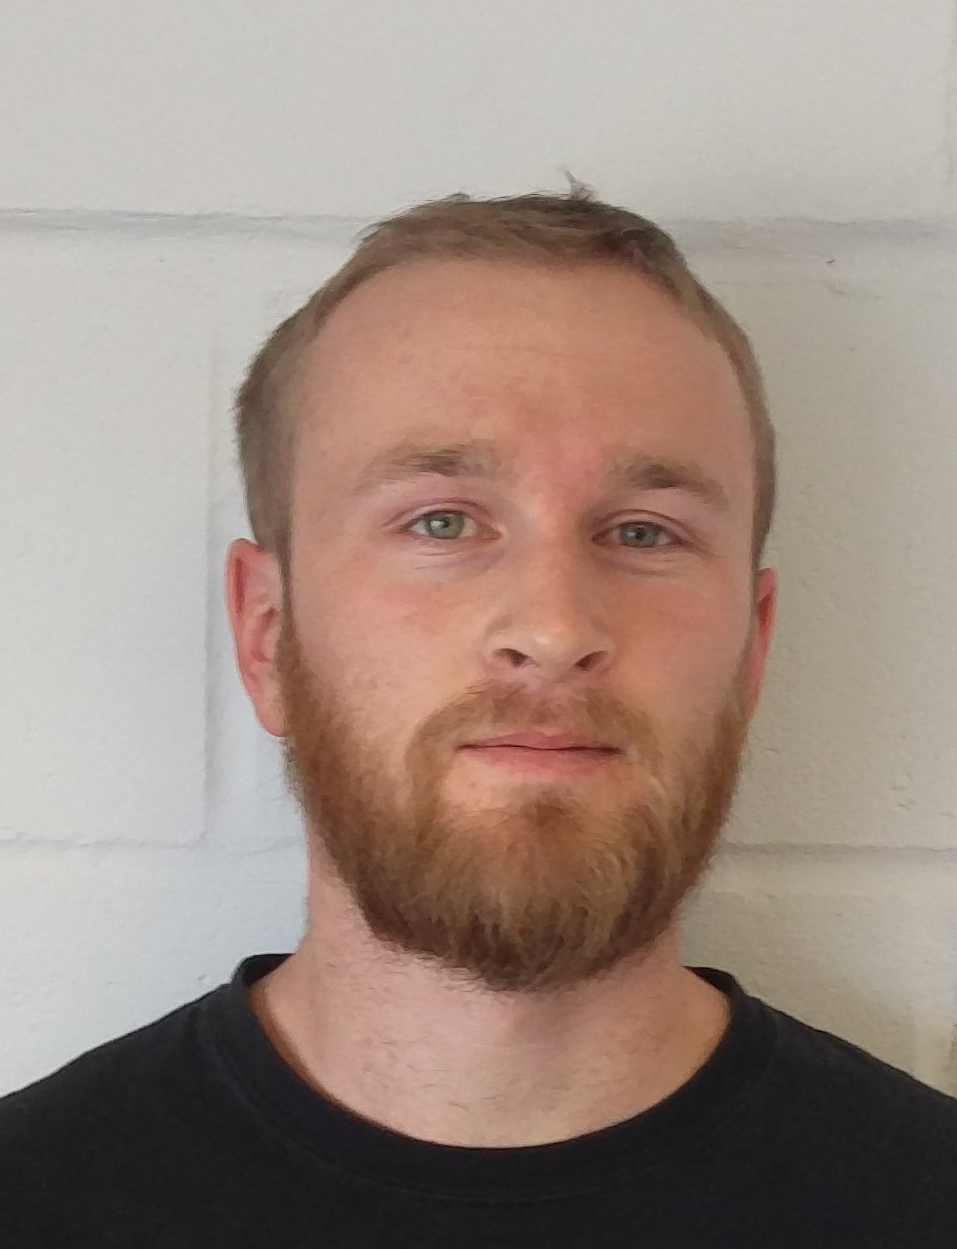
\includegraphics[trim=0 0 0 0,clip,height=1.05cm]{figure/mug.jpg}
  \end{column}
  \end{columns}
  {\color{slfcolor}\hrule height 1pt\vspace{0.1cm}}
\end{beamercolorbox}%
}

% setup the navigation in footbox
% first set some button colors
\newcommand{\buttonactive}{\setbeamercolor{button}{bg=wslcolor,fg=white}}
\newcommand{\buttonpassive}{\setbeamercolor{button}{bg=slfcolor,fg=white}}
% now set up that the one active one gets the new color.
\newcommand{\secvariable}{nothing}
% therefore we write before each section (well, everything which should be part of the navi bar)
% the variable \secvariable to any name which is in the next function ...
\newcommand{\mysection}[1]{\renewcommand{\secvariable}{#1}
}
% ... compaired to strings in the following navibar definition ...
\newcommand{\tocbuttoncolor}[1]{%
 \ifthenelse{\equal{\secvariable}{#1}}{%
    \buttonactive}{%
    \buttonpassive}
 }
% ... here we start to set up the navibar. each entry is calling first the function \tocbuttoncolor with the argument which should be tested for being active. if active, then change color. afterwards the button is draw. so to change that, you need to change the argument in \toc..color, the first in \hyperlink and before each frames definition... A bit messed up, but works...
\newlength{\buttonspacingfootline}
\setlength{\buttonspacingfootline}{-0.2cm}
\setbeamertemplate{footline}
{\leavevmode
\begin{beamercolorbox}[width=1\paperwidth]{head title}
  {\color{slfcolor}\hrule height 1pt}
  \vspace{0.05cm}
  % set up the buttons in an mbox
  \centering \mbox{
    \tocbuttoncolor{intro}
    \hyperlink{intro}{\beamerbutton{Introduction}}
    \tocbuttoncolor{trial_shear}
    \hspace{\buttonspacingfootline}
      \hyperlink{trial_shear}{\beamerbutton{Trials results}}
    \tocbuttoncolor{plan}
    \hspace{\buttonspacingfootline}
      \hyperlink{plan}{\beamerbutton{Deployment plan}}
    \tocbuttoncolor{qc}
    \hspace{\buttonspacingfootline}
      \hyperlink{qc}{\beamerbutton{Data qc}}
    \tocbuttoncolor{tech}
    \hspace{\buttonspacingfootline}
      \hyperlink{tech}{\beamerbutton{Tech specs}}
    % this last one should normaly not be used... it will open the preferences to change the 
    % behaviour of the acrobat reader in fullscreen -> usefull in pico...
    \setbeamercolor{button}{bg=white,fg=black}
    % for presentation
    %\hspace{-0.1cm}\Acrobatmenu{FullScreenPrefs}{\beamerbutton{\#}}
    % for upload
    
     
\Acrobatmenu{FullScreenPrefs}{\vspace{0.3cm}\hspace{0.24cm}\mbox{%
      \includegraphics[height=0.04\textheight,keepaspectratio]{%
	  figure/CreativeCommons_Attribution_License}%
	  }}
   }
    \vspace{0.05cm}
\end{beamercolorbox}%
}



\begin{document}


%%%%%%%%%%%%%%%%%%%%%%%%%%%%%%%%%%%%%%%%%%%%%%%%%%%%%%%%%%%%%%%%%%%%%%%%%%
\mysection{intro}
%%%%%%%%%%%%%%%%%%%%%%%%%%%%%%%%%%%%%%%%%%%%%%%%%%%%%%%%%%%%%%%%%%%%%%%%%%
\begin{frame}\label{\secvariable}
\usebeamerfont{bodytext}
\justifying

\vspace*{-1.2mm}    

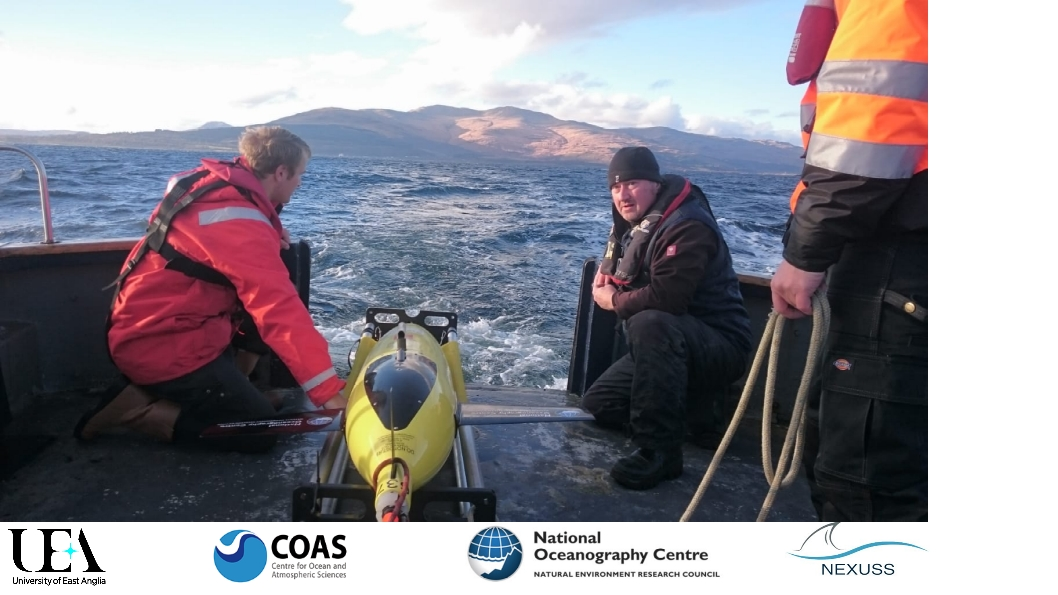
\includegraphics[trim=0 0 100 5,clip,width=\paperwidth]{figure/splash.jpg}


\end{frame}

%%%%%%%%%%%%%%%%%%%%%%%%%%%%%%%%%%%%%%%%%%%%%%%%%%%%%%%%%%%%%%%%%%%%%%%%%%
\mysection{trial_shear}
%%%%%%%%%%%%%%%%%%%%%%%%%%%%%%%%%%%%%%%%%%%%%%%%%%%%%%%%%%%%%%%%%%%%%%%%%%
\begin{frame}\label{\secvariable}
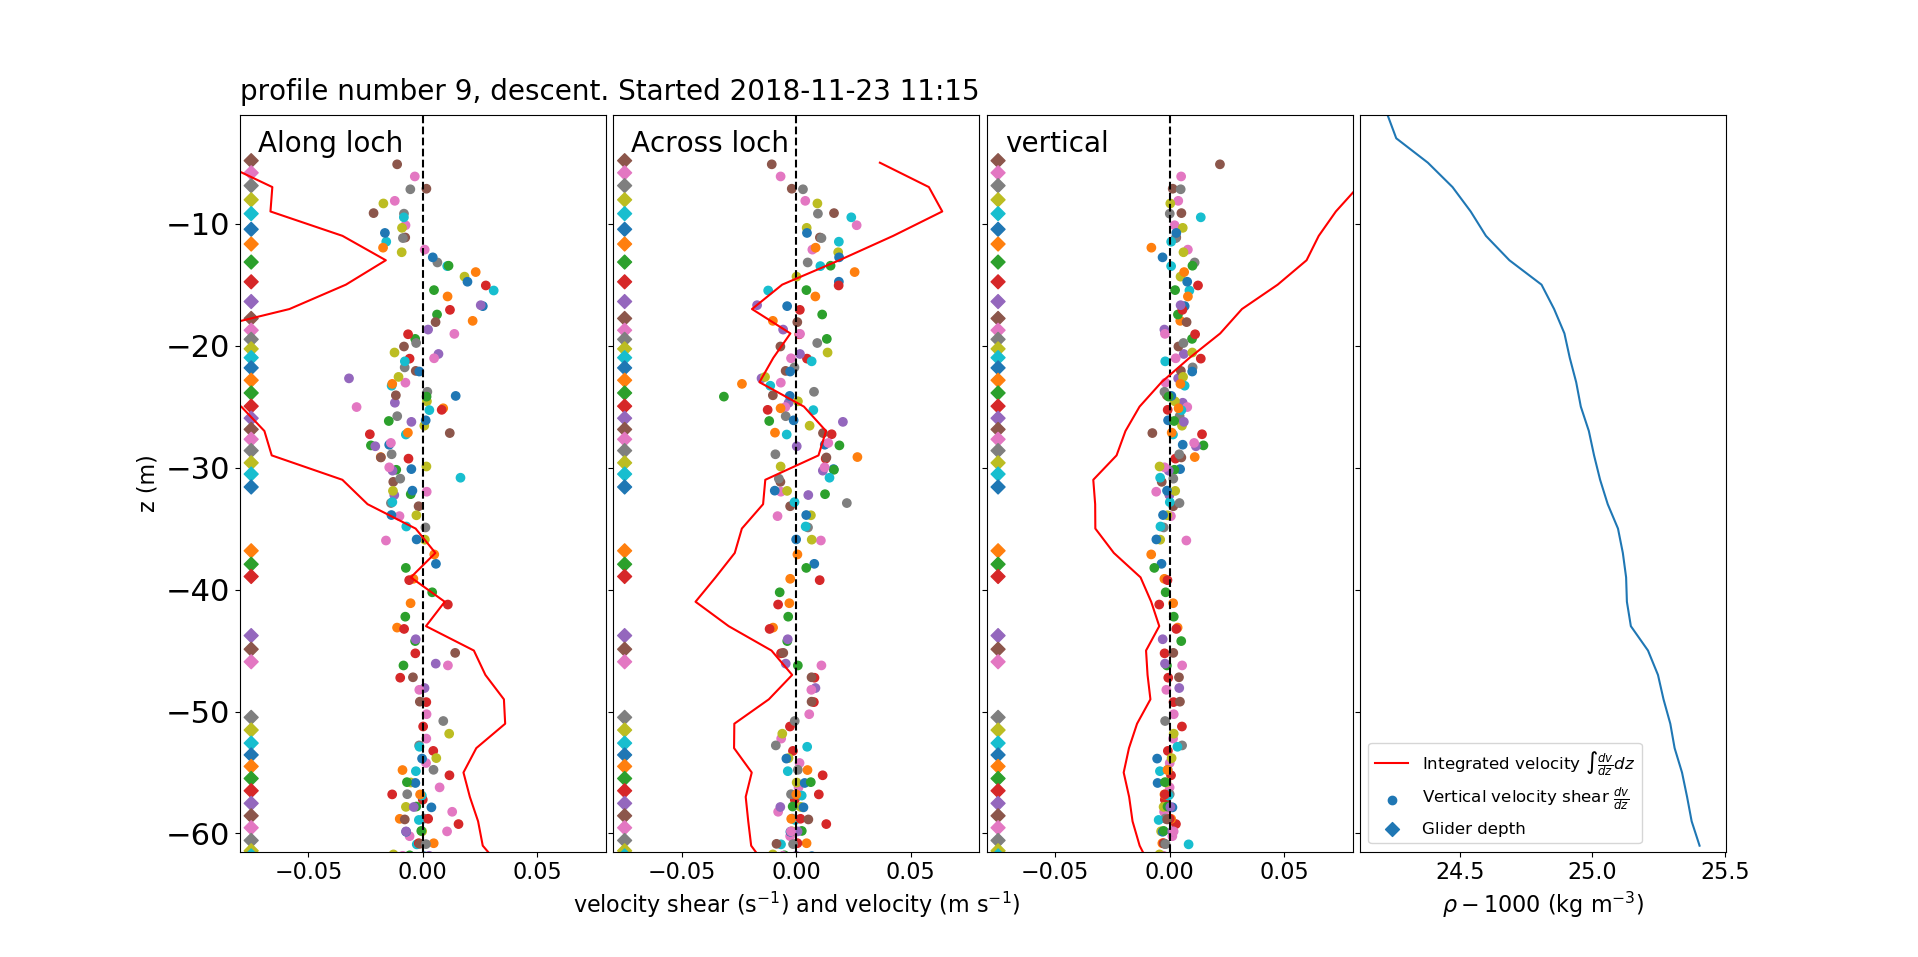
\includegraphics[trim=70 20 80 80,clip,width=\paperwidth]{figure/95_qc.png}

\begin{itemize}
\item Vertical shear of horizontal velocity coherent between ensembles
\item Strong along loch shear across pycnocline
\end{itemize}
  
\end{frame}


\begin{frame}\label{sawtooth}
\vspace*{-1.2mm}    
\begin{center}
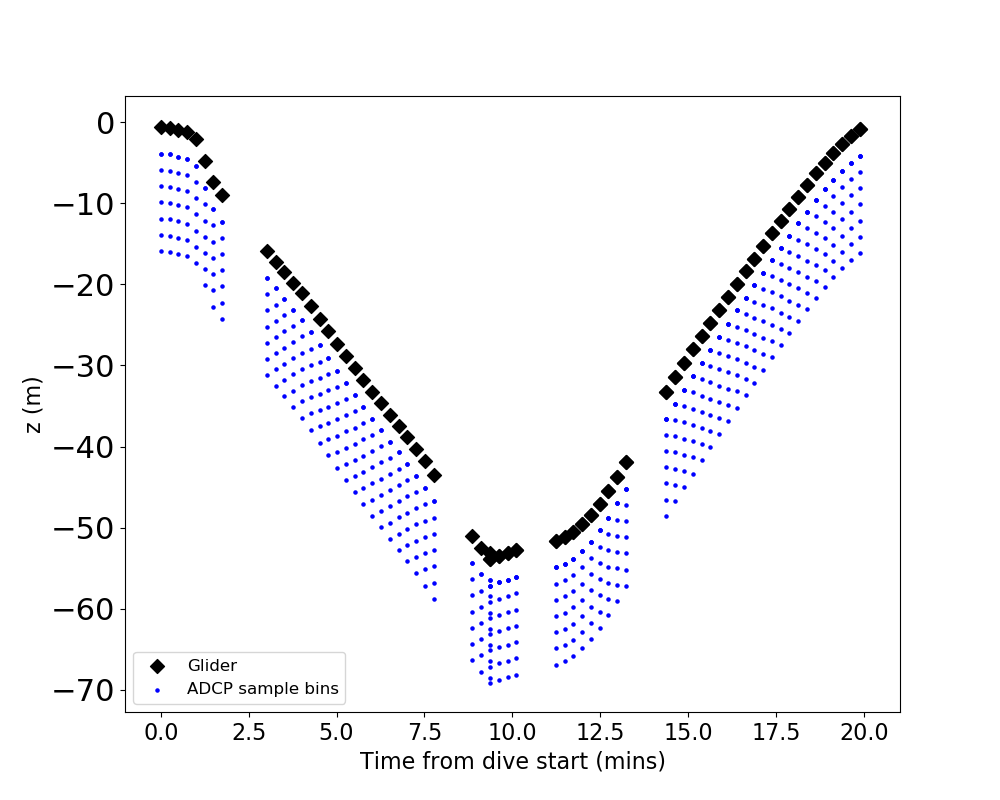
\includegraphics[trim=0 0 0 50,clip,width=0.8\paperwidth]{figure/sawtooth.png}
\end{center}

\vspace*{-5.2mm}
\begin{columns}
\begin{column}[t]{0.9\textwidth}
Dive profile from trials with glider depth and bins out to 15 m plotted
\end{column}
\end{columns}


  
\end{frame}

\begin{frame}\label{3_dives}
\vspace*{-1.2mm}    
\begin{center}
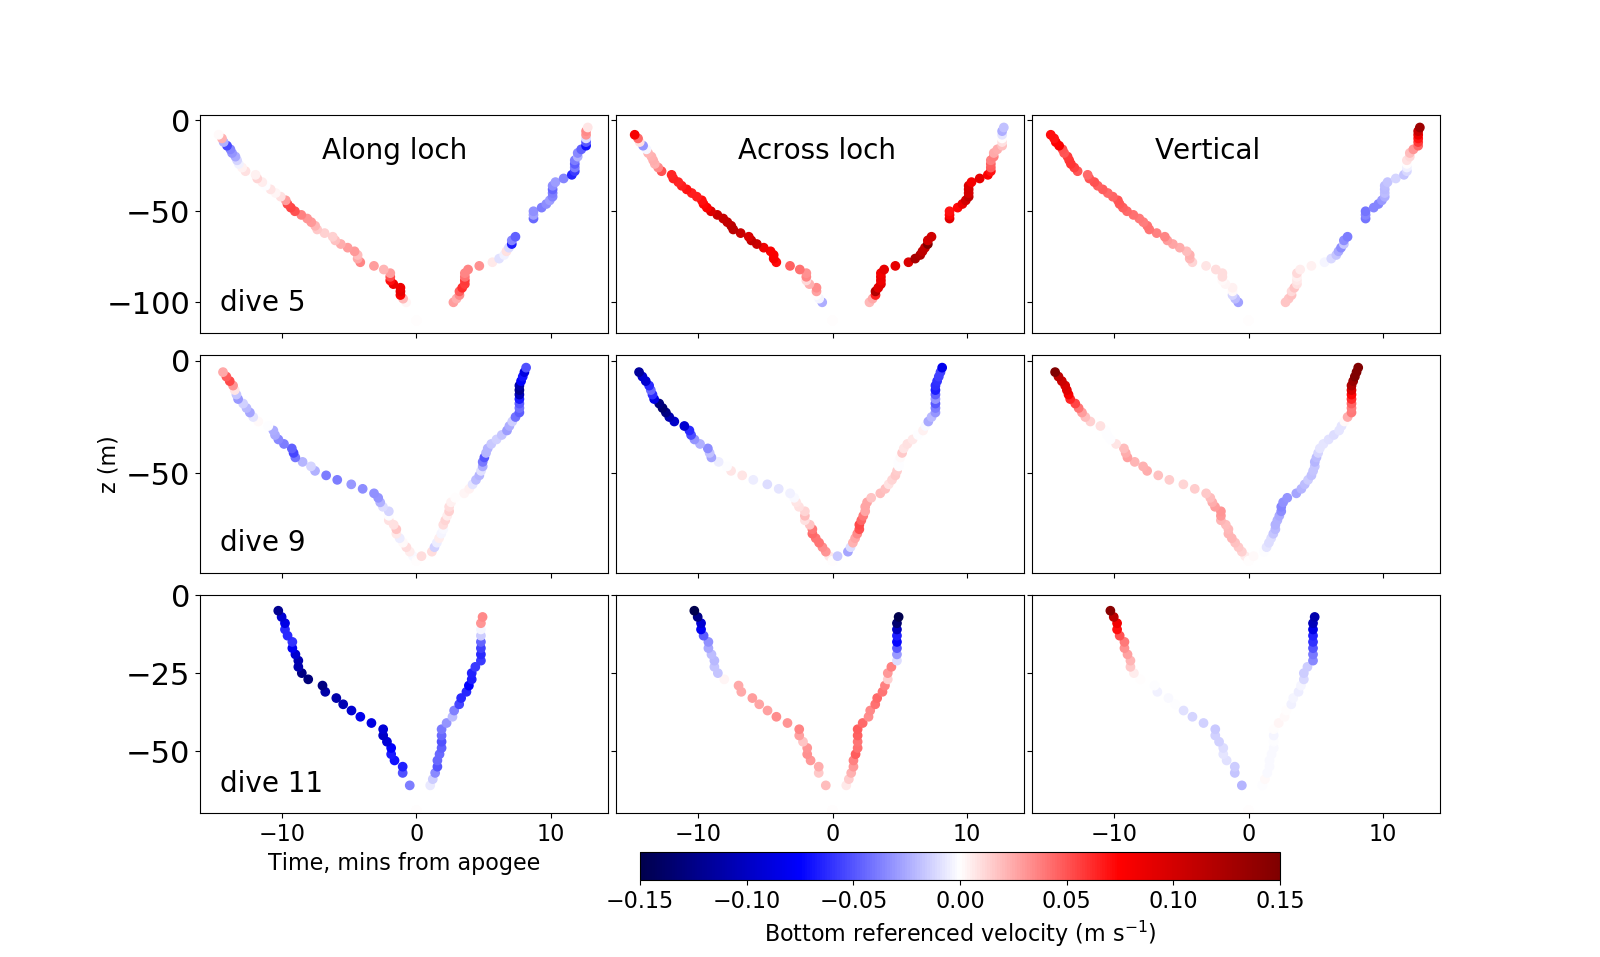
\includegraphics[trim=0 0 0 50,clip,width=\paperwidth]{figure/diveclimb_vel9.png}
\end{center}

\vspace*{-5.2mm}
\begin{columns}
\begin{column}[t]{0.9\textwidth}
Good agreement for horizontal velocities between descents and ascents
\end{column}
\end{columns}



  
\end{frame}



%%%%%%%%%%%%%%%%%%%%%%%%%%%%%%%%%%%%%%%%%%%%%%%%%%%%%%%%%%%%%%%%%%%%%%%%%%
\mysection{plan}
%%%%%%%%%%%%%%%%%%%%%%%%%%%%%%%%%%%%%%%%%%%%%%%%%%%%%%%%%%%%%%%%%%%%%%%%%%
\begin{frame}\label{\secvariable} %%Eine Folie
\vspace{-0.3cm}
\begin{center}
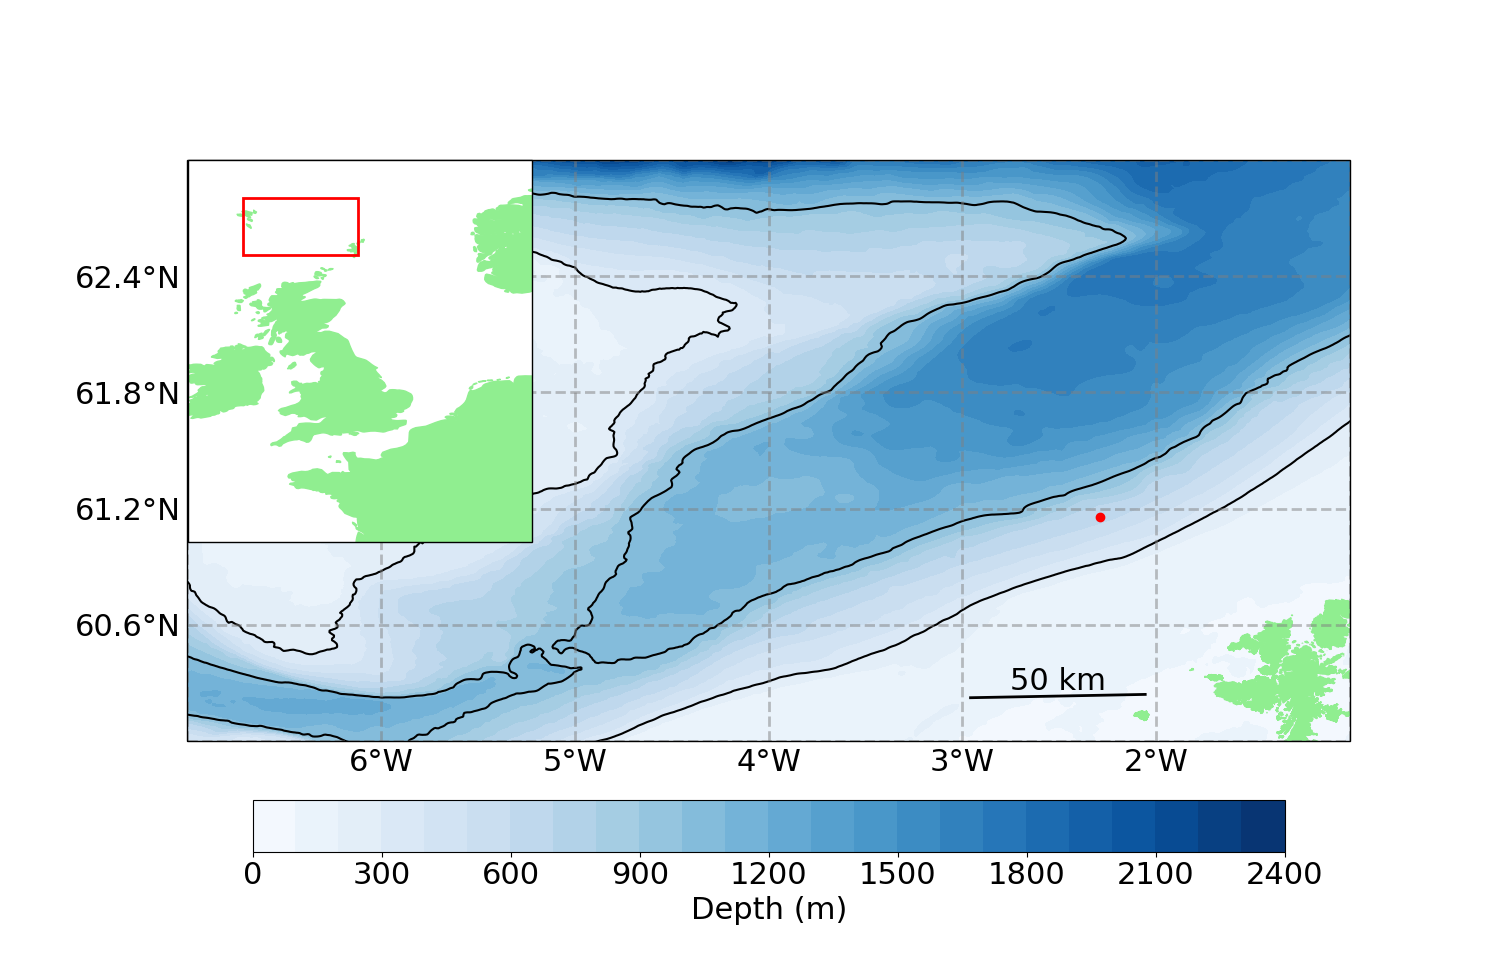
\includegraphics[trim=0 10 0 110,clip,width=1\textwidth,keepaspectratio]{%
figure/basemap.png}
\end{center}
\begin{columns}
\begin{column}[t]{0.9\textwidth}
Deployment to the Faroe Shetland Channel April 2019 in conjunction with ADCP mooring and PIES \hyperlink{fsc_shear}{\beamerbutton{see expected conditions}}
\end{column}
\end{columns}
\end{frame}


\begin{frame}\label{fsc_shear}
\vspace*{-10mm}    
\begin{center}
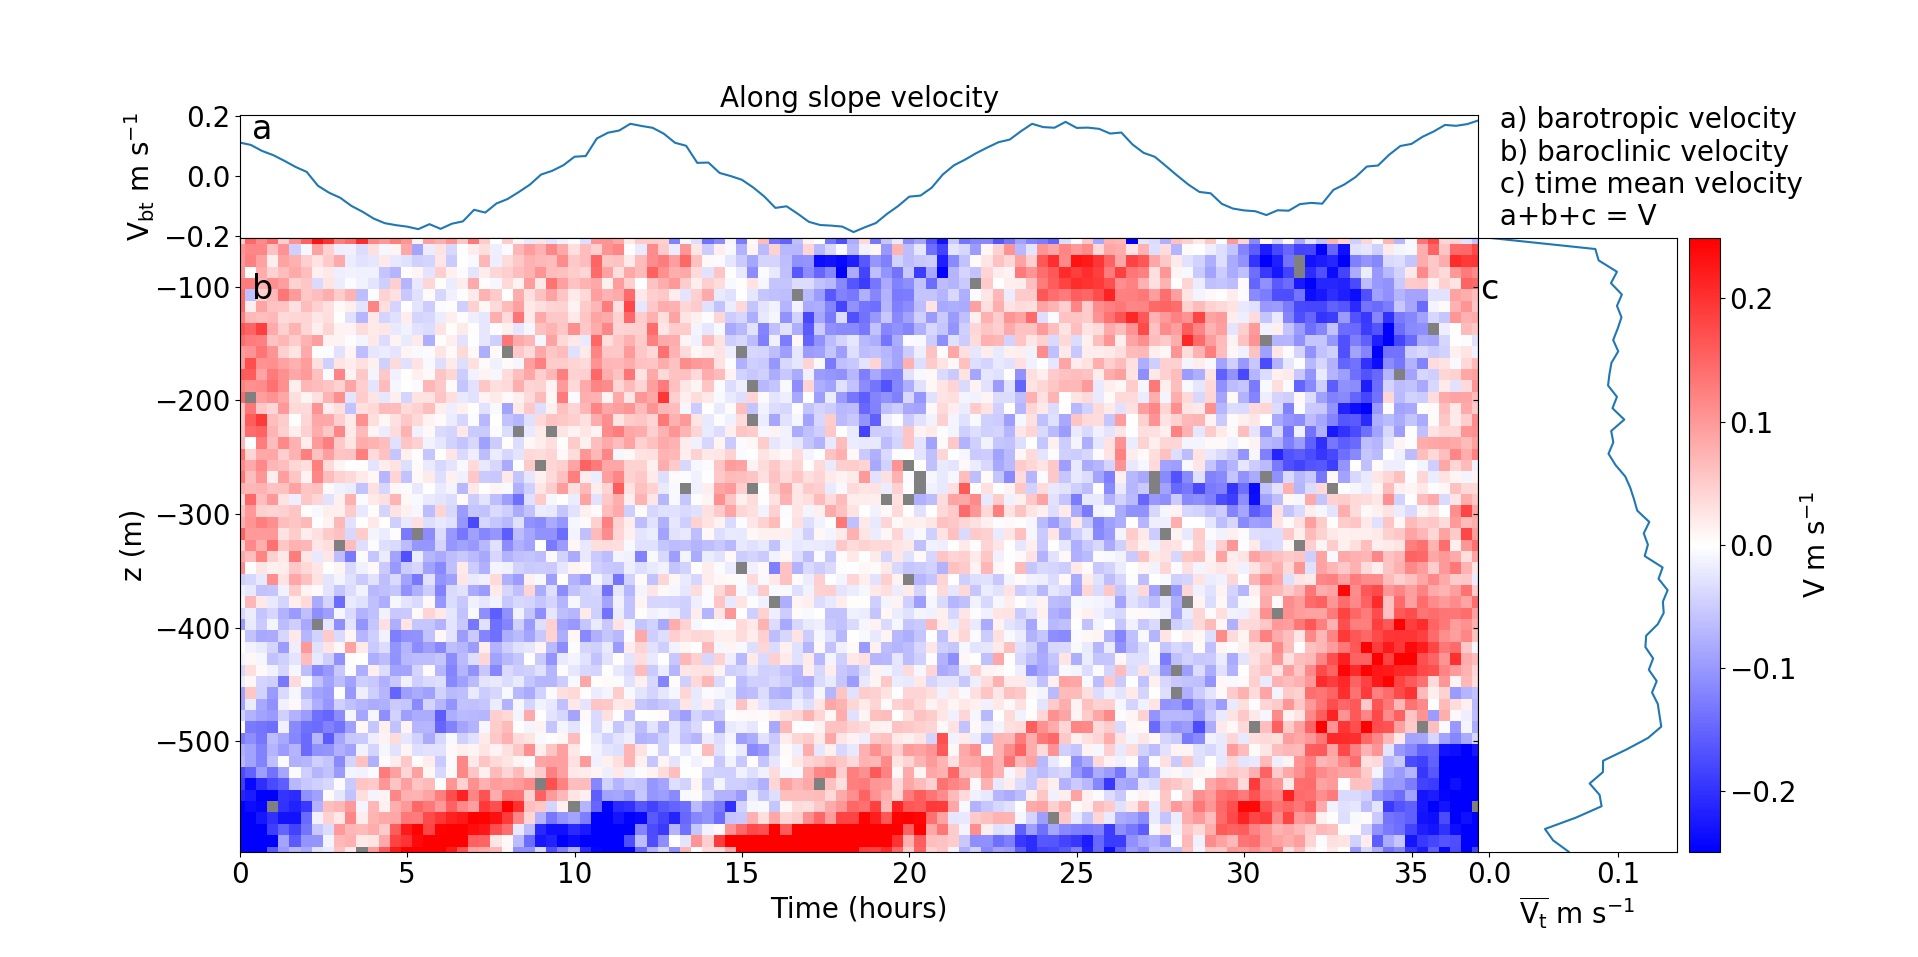
\includegraphics[trim=20 20 20 60,clip,width=\paperwidth]{figure/adcp_fsc.png}
\end{center}
\vspace*{-5mm}    
\begin{columns}
\begin{column}[t]{0.9\textwidth}
Tidal currents of $0.2\ \mathrm{m\ s^{-1}}$ and a mean flow of $0.1\ \mathrm{m\ s^{-1}}$ bottom intensified baroclinic tidal flows will be a good test of the ADCP glider.  

ADCP data courtesy of Bee Berx, Marine Scotland Science
\end{column}
\end{columns}
 
\end{frame}
%%%%%%%%%%%%%%%%%%%%%%%%%%%%%%%%%%%%%%%%%%%%%%%%%%%%%%%%%%%%%%%%%%%%%%%%%%
\mysection{qc}
%%%%%%%%%%%%%%%%%%%%%%%%%%%%%%%%%%%%%%%%%%%%%%%%%%%%%%%%%%%%%%%%%%%%%%%%%%
\begin{frame}\label{\secvariable}
\ \ Quality control  and calculation steps
\begin{itemize}
\item Discard cells where glider attitude causes beam miss of $> 1$ m \hyperlink{flight_envelope}{\beamerbutton{see plot}}
\item Discard cells where the ping correlation is less than 50\%
 \hyperlink{ping_corr}{\beamerbutton{see plot}}
\item Rotate from beam coordinates to East-North-Up using data from attitude sensors and compass on the ADCP
\item Calculate shear between each remaining adjacent cell
\item Average shear data in 2 m vertical bins
\item Integrate shear to get relative velocity profiles
\item Reference relative velocity profiles using dive average current from the glider for "absolute" velocity profiles
\item What if we don't use quality control? \hyperlink{no_qc}{\beamerbutton{see plot}}
\end{itemize}
\end{frame}


\begin{frame}\label{flight_envelope}
\vspace{-0.3cm}
\begin{center}
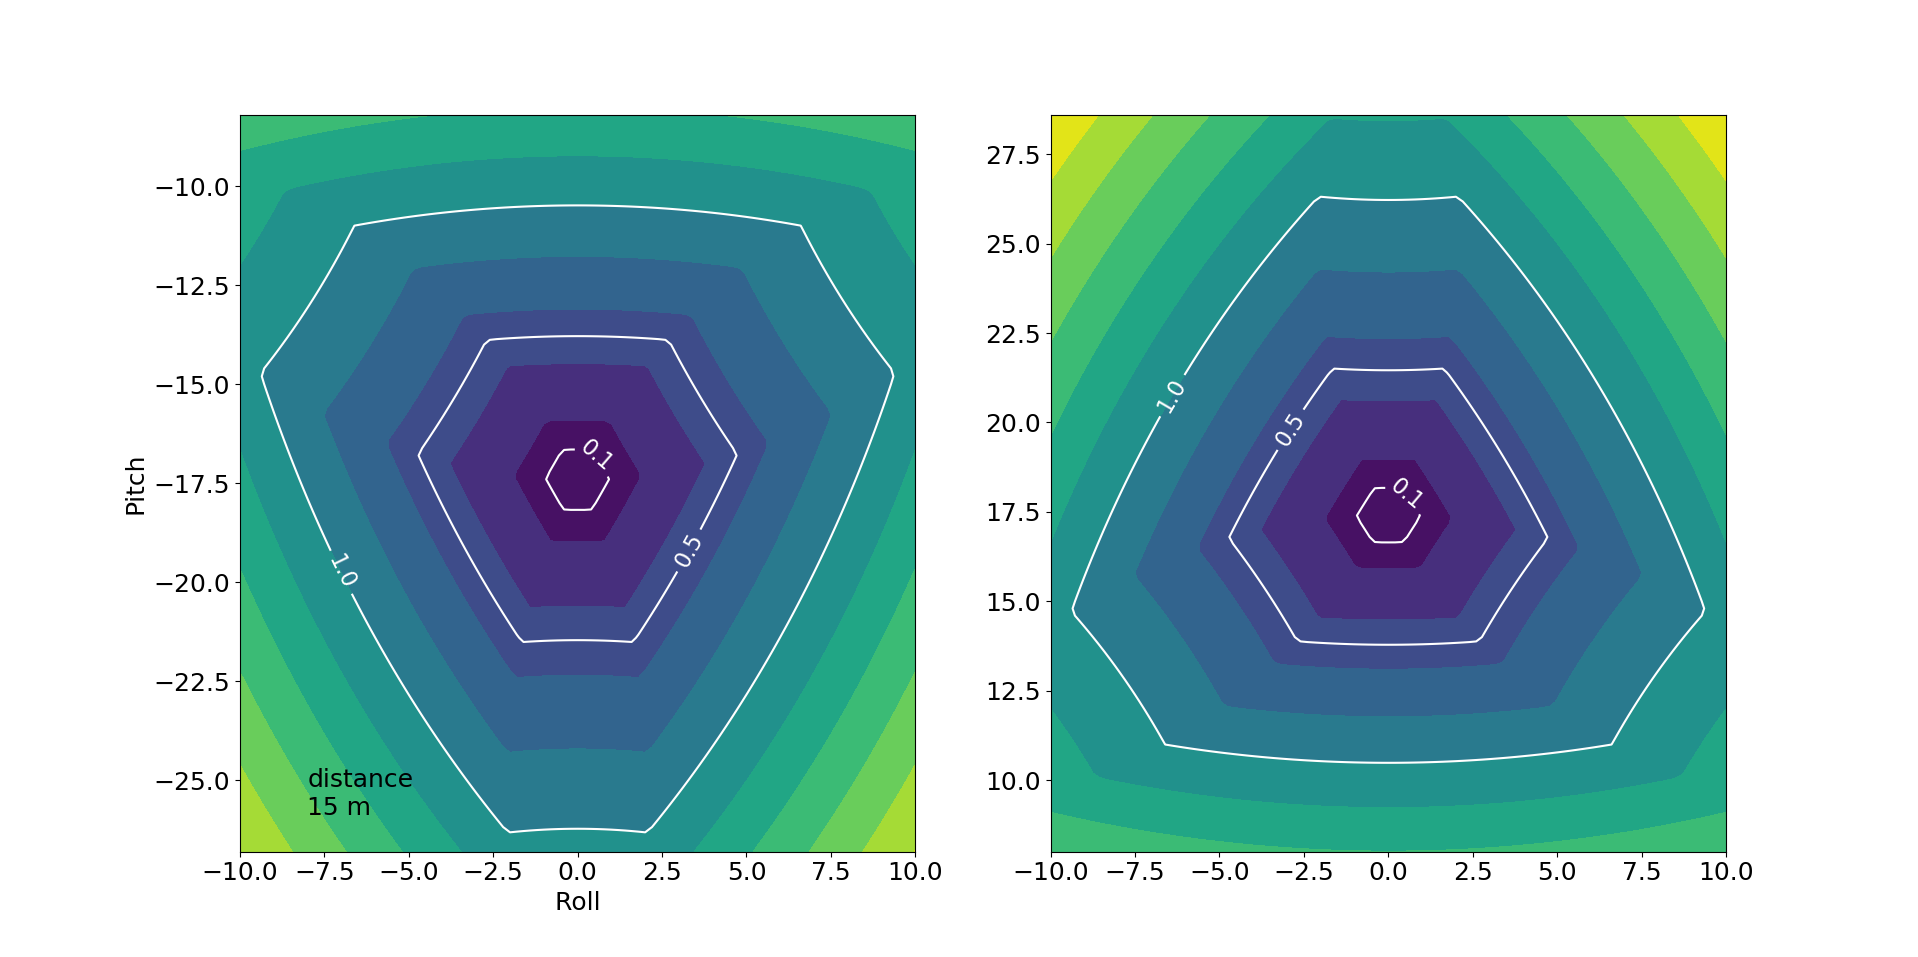
\includegraphics[trim=0 10 0 50,clip,width=1\textwidth,keepaspectratio]{%
figure/flight_aim.png}
\end{center}
\vspace{-0.3cm}
\begin{columns}
\begin{column}[t]{0.9\textwidth}
Flight angles affect the vertical location of the three beams. Plot shows the vertical distance between beams sampling a cell 15 m from the glider over a range of pitch and roll angles. Perfect sampling (0 m beam miss) is achieved at $\pm17.3^{\circ}$ pitch $0^{\circ}$ roll
\end{column}
\end{columns}
\end{frame}

\begin{frame}\label{ping_corr}
\vspace{-0.3cm}
\begin{center}
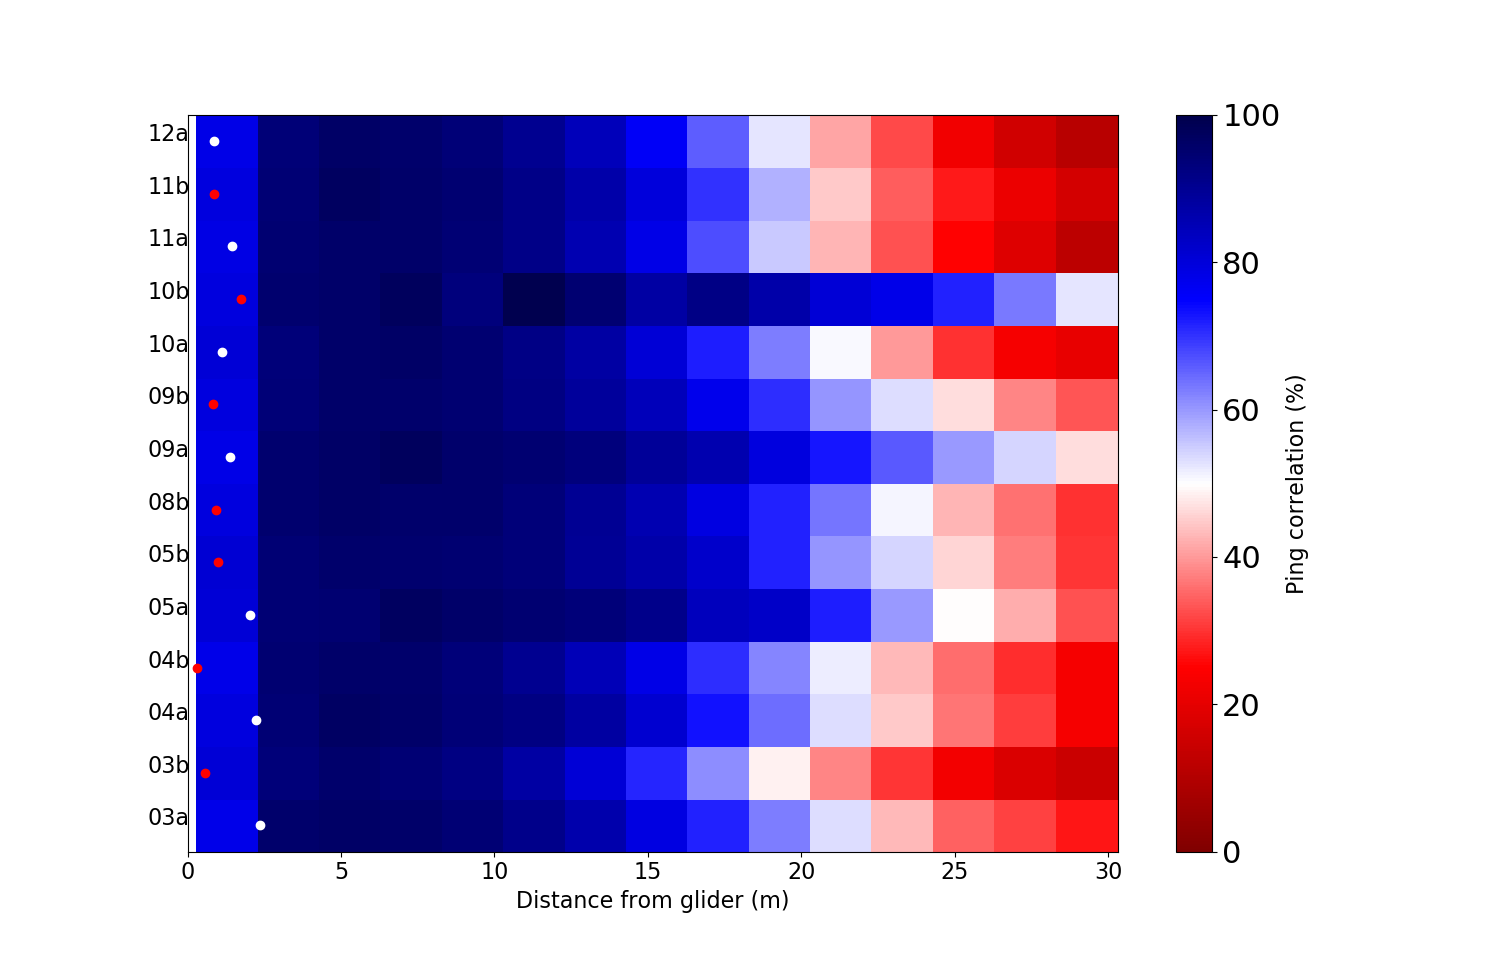
\includegraphics[trim=0 10 0 50,clip,width=0.8\textwidth,keepaspectratio]{%
figure/corr.png}
\end{center}
\vspace{-0.3cm}
\begin{columns}
\begin{column}[t]{0.9\textwidth}
Dots are vertical missmatch of  beams at 15 m from glider. white for descent, red for ascent. Closer to 0 = better flight
\end{column}
\end{columns}
\end{frame}

\begin{frame}\label{no_qc}
\vspace{-0.3cm}
\begin{center}
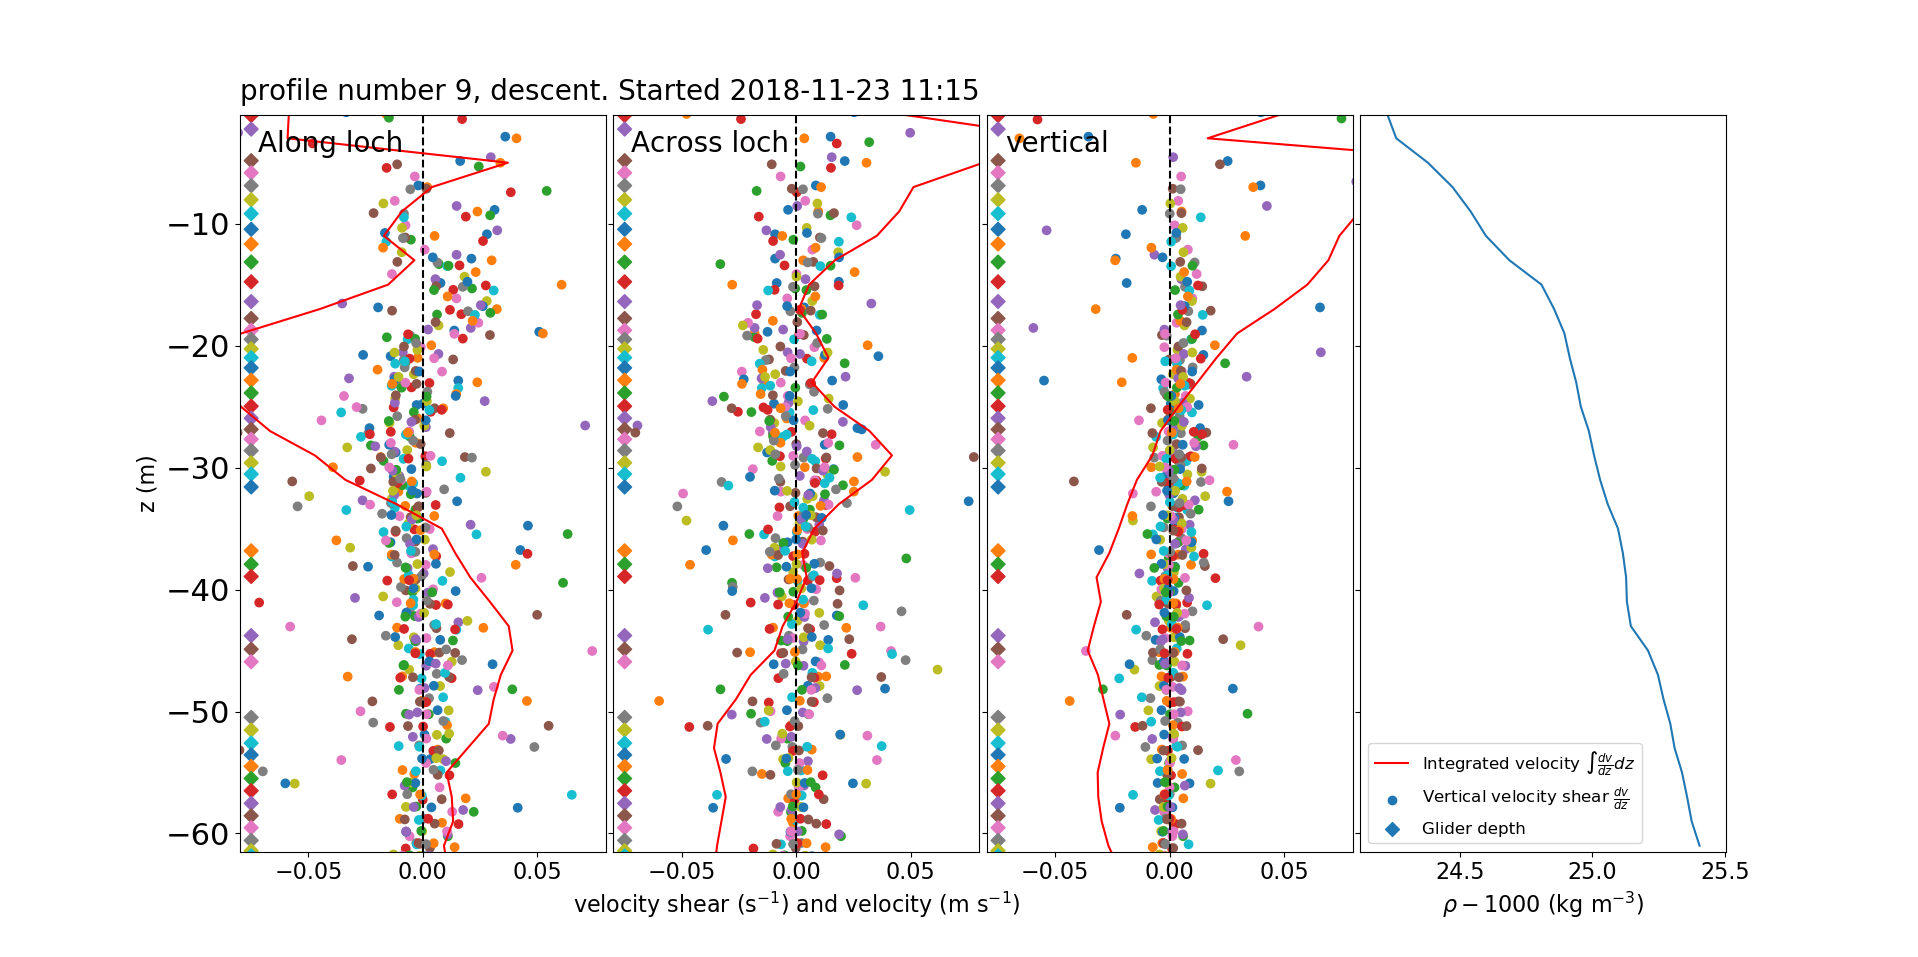
\includegraphics[trim=70 20 80 80,clip,width=\paperwidth]{figure/95_noqc.png}
\end{center}
\begin{columns}
\begin{column}[t]{0.9\textwidth}
The same data as the introduction, without quality control steps
\end{column}
\end{columns}
\end{frame}


%\hyperlinkslidenext{\beamerbutton{next}}


%%%%%%%%%%%%%%%%%%%%%%%%%%%%%%%%%%%%%%%%%%%%%%%%%%%%%%%%%%%%%%%%%%%%%%%%%%
\mysection{tech}
%%%%%%%%%%%%%%%%%%%%%%%%%%%%%%%%%%%%%%%%%%%%%%%%%%%%%%%%%%%%%%%%%%%%%%%%%%
\begin{frame}\label{\secvariable}

  \vspace{-1.5cm}
\ Seaglider max depth 1000m , vertical velocity 0.1 m/s

\ ADCP spec:
\begin{itemize}
\item Sampling frequency 1 MHz 
\item Range 30 m (max) 10-15 m (typical)
\item 3 downward looking beams at 30 degrees from vertical 
\item Cell size 2 m
\item 2 second ensemble of 8 pings every 30 seconds
\item Expected endurance 6 weeks
\end{itemize}
  
\begin{columns}
\begin{column}[t]{0.9\textwidth}
\usebeamerfont{bodytext}PICO adapted from the template by Anselm K\"ohler found here: \\ \texttt{https://github.com/snowtechblog/pico-latex-presentation}
\end{column}
\end{columns}
\end{frame}



\end{document}
